More emphasis on the localisation of events
Why do we use trajectories? Because we learn more about the location of the user  
Points have a semantics of trajectories so we can group them as trajectories for better positioning

Add an example

how good we estimate the location of users from their network activtiy. Users move and genereate trajectories therefore the rceords have a semantics of trajectories so we group the points into trajectories and then we can benefit from prior work don in trajectory mining for localisation of users. 
Only for evaluation purposes we consider them as trajectories


We compare ground truth GPS trajectories to trajectories of CDR events for the same time window in a distributed fashion as shown in Figure \ref{fig:problem}. 
\begin{figure}[h]
    \centering
    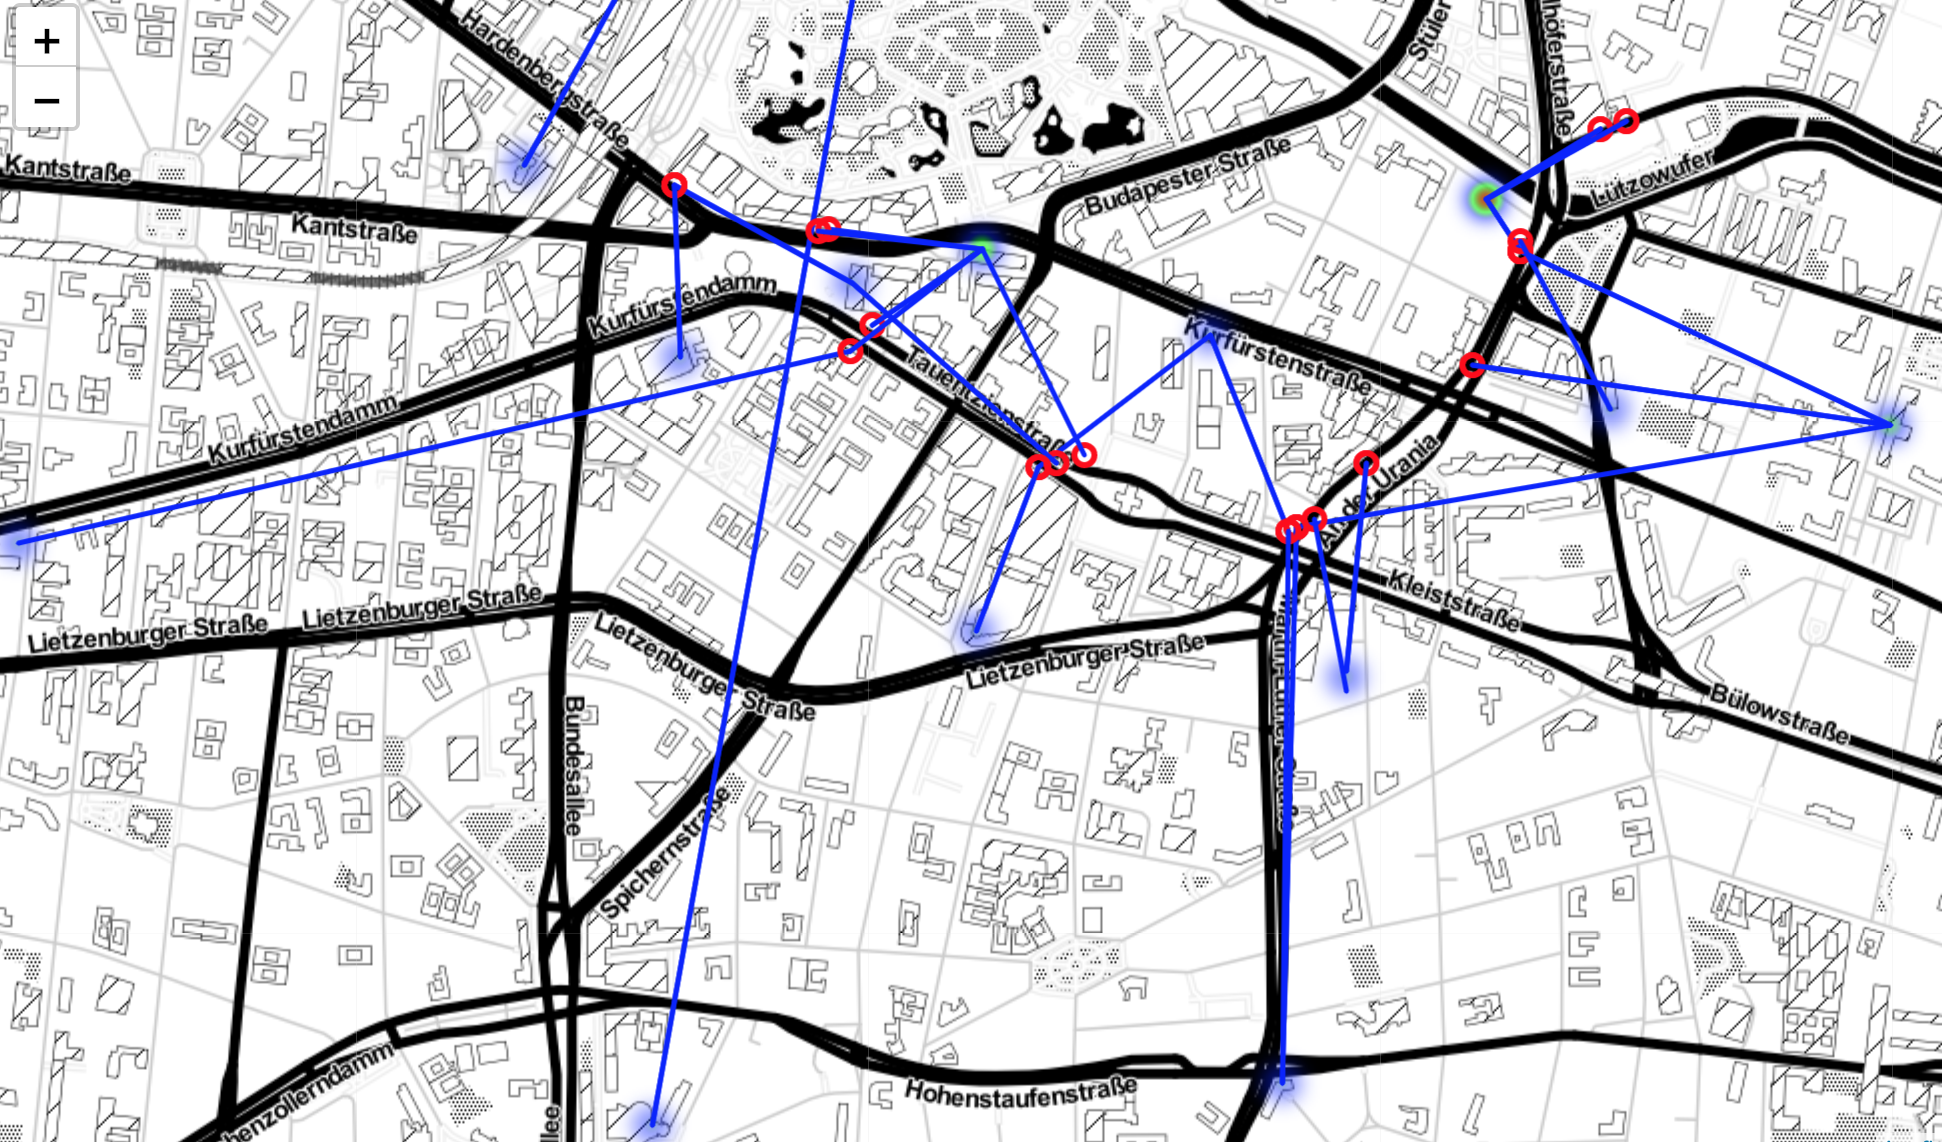
\includegraphics[width=0.45\textwidth]{images/localization_eval.png}
    \caption{Problem illustration (Notation: red circle - GPS observation, heat map - CDR location, i.e. location of assigned cell to CDR event, blue line - distance of GPS and CDR location.)}
    \label{fig:problem}
\end{figure}

To evaluate cellular network event based customer localization we calculate the Euclidean distance and several statistics of the pairwise distances between ground truth GPS trajectories and mobile network event trajectories. The Haversine distance is used to define the spatial distance between points. In the mobile network event trajectory, the location information is obtained from cell map data set.

For these calculations the number of CDR and GPS observations need to match. We join the two trajectories on the timestamp, namely for each CDR event we select the closest GPS observation in time.

\begin{definition}
A for any two points on a sphere, the Haversine formula determines the spatial distance between the two points \cite{haversine}:
    \[\Delta_{x} = x_{2} - x_{1}\]
    \[\Delta_{y} = y_{2} - y_{1}\]
    \[a = (\sin(\Delta_{y}/2))^2 + \cos{(y_{1})} * \cos{(y_{2})} * (\sin{(\Delta_{x}/2)})^2 \]
    \[c = 2 * \arcsin{(\min{1,\sqrt{a}})}\]
    \[d(P_{1}, P_{2}) = R * c\]
    where $R$ is the radius of the Earth and $x_{i}, y_{i}$ is the longitude, latitude values of $P_{i}$ in radians.
\end{definition}

Given a set of distance observations with size $n$, we consider $\{d_{1}, d_{2}, ..., d_{n}\}$ as $n$ independent identically distributed (i.i.d) random variables, each corresponding to one randomly selected observation and having the distribution of the population. Then we can calculate the following descriptive statistics for the sample:
\begin{itemize}
    \item mean:
     \[ \overline {d} = \frac{\sum_{i=1}^{n} d_{i}}{n}\]
     \item standard deviation:
    \[ \sigma={\sqrt {\frac {\sum _{i=1}^{n}(d_{i}-{\overline {d}})^{2}}{n-1}}}\]
    \item sum:        
    \[s = \sum_{i=1}^{n} d_{i}\]
\end{itemize}

Note that $\{d_{1}, d_{2}, ..., d_{n}\}$ are the spatial distances between pairs of points from the trajectories. For each pair of points, $d_{i} = d(P_{i},\Tilde{P_{i}})$ and $n$ is the number of points in the trajectories.

The \textit{Euclidean distance} (or inverse similarity) measure between two trajectories is used in this analysis:
\[D(T,\Tilde{T}) = \sqrt{\sum_{i=1}^{n} (d(P_{i},\Tilde{P_{i}}))^{2}}\]

%\begin{itemize}
    %\item 
%    \item \textit{dynamic time warping distance} as in \cite{traj-sim-rev}:
%    \[
%        D(T,\Tilde{T}) =
%        \begin{cases}
%            0, \text{if } n=m=0 \\
%            \infty,\text{if }  n=0 \text{ or } m=0 \\
%            d(h(T), h(\Tilde{T})) + \min 
%            \begin{cases}  
%                D(r(T),\Tilde{T}) \\
%                D(T,r(\Tilde{T})) \\
%                D(r(T),r(\Tilde{T})) 
%            \end{cases}
%        \end{cases}
%    \]
%    where $h(.)$ returns the first point in the trajectory and $r(.)$ returns all except the first one.
%\end{itemize}



